\section{\textit{Mobile App}}

Este capítulo descreve o desenvolvimento e implementação da aplicação móvel. O mesmo é composto por uma introdução, seguindo-se a apresentação da navegação na aplicação e a arquitetura da mesma. Por fim, discute-se a implementação de cada sub-módulo da arquitetura.

\bigskip \bigskip

O componente aplicação móvel funciona como interface para o tipo de utilizador mais comum (Voluntário) e foi desenvolvida para a plataforma Android.

\par \bigskip \bigskip

Este módulo contém alguns requisitos chave que são necessários para garantir a usabilidade da mesma por parte dos seus utilizadores. Alguns dos requisitos são:

\begin{itemize}
	\item garantir que possam ver os \textit{posts} e eventos que estão registados na plataforma;
	\item possibilitar que possam gostar \textit{posts}, seguir utilizadores e registarem-se em eventos (ou seja, implementar a interação de uma rede social);
	\item existência do conceito sessão de maneira a terem uma experiência personalizada, e possibilitar que possam editar o seu perfil, efetuar \textit{posts}, entre outros.
\end{itemize}

\bigskip

Tal como já foi referido anteriormente, foi tomada a decisão de implementar esta aplicação no sistema operativo Android seguindo as orientações dadas pelo Android Jetpack e um conjunto de bibliotecas auxiliares (como o Volley e o Glide).

\bigskip \bigskip

\subsection{Navegabilidade e utilização da \textit{App}}

\bigskip

A interface gráfica com o utilizador foi cuidadosamente desenhada e testada de modo a que a sua utilização fosse o mais intuitiva possível. O grafo de navegação é ilustrado na figura 7.

\newpage

\begin{figure}[h]
	\centering
	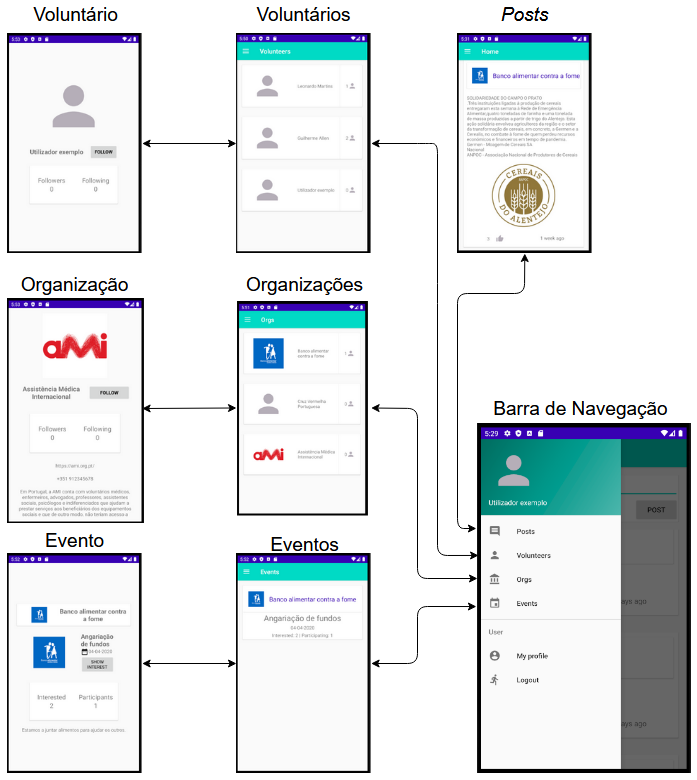
\includegraphics[scale=.55]{app_navigation.png}
	\caption{Grafo de navegação}
\end{figure}

Foram desenvolvidas quatro vistas principais de pesquisa (\textit{posts}, voluntários, organizações e eventos) que apresentam os dados existentes na plataforma. Existem também vistas detalhadas para estes mesmos índices (exceto \textit{posts}) para que o utilizador possa ver os detalhes destes dados.

\bigskip

\subsection{Sessão}

De maneira a garantir uma experiência personalizada para cada cliente deste módulo, foram desenvolvidos ecrãs e mecanismos de de registo e autenticação de clientes.

\bigskip

A partir do momento que um cliente da aplicação se encontre autenticado, certas operações como ``gostar'' um \textit{post} ou seguir um utilizador passam a estar disponíveis e determinados ecrãs irão ter uma vista personalizada, tal como exemplificado na figura 8.

\newpage

\begin{figure}[h]
	\centering
	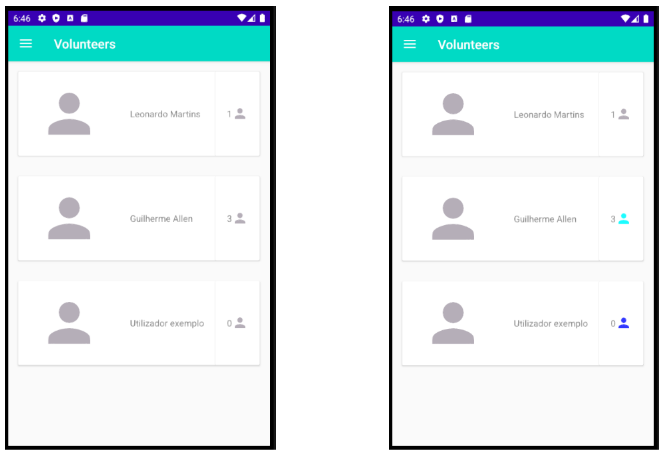
\includegraphics[scale=.70]{unauthenticated_vs_authenticated}
	\caption{Representação do ecrã ``Voluntários'' no estado não autenticado (esquerda) e no estado autenticado (direita) como o utilizador ``Utilizador exemplo''.}
\end{figure}

\subsection{Arquitetura}

A arquitetura da aplicação é constituída por três sub-módulos principais: UI (User Interface), API e Modelo.

\medskip

Enquanto que a UI é responsável por conter as implementações dos mais variados aspetos da interface de utilizador (como atividades, fragmentos, navegação e outros elementos), a API trata a comunicação entre a aplicação e a Web API. Por fim, o Modelo define a estrutura dos dados fornecidos pela API e utilizados na UI assim como a implementação de uma \textit{cache} de maneira a partilhar estes dados e reduzir o número de pedidos efetuados à Web API.

\subsection{Implementação de Sessão}

Tendo em conta que o conceito de sessão foi implementado na Web API através da tecnologia Passport.js (que funciona à base de \textit{cookies}), foi necessário redefinir algumas infra-estruturas da biblioteca Volley (utilizada para efetuar pedidos HTTP) de maneira a que, quando o utilizador estiver autenticado na aplicação, os pedidos efetuados pela mesma contenham a informação necessária para a Web API conseguir reconhecer o utilizador.

\medskip

De maneira a que a representação dos vários ecrãs da aplicação seja dinâmica consoante a sessão do utilizador, é definido e utilizado um objeto Sessão, acessível por todas as classes do projeto, que contém informações relativamente ao voluntário autenticado.

\subsection{\textit{User Interface}}

Este sub-módulo engloba todos os componentes do projeto que são responsáveis por representar os dados da aplicação. Este é constituído por:

\begin{itemize}
	\item implementações de ecrãs, quer sejam atividades ou fragmentos. É de notar que para cada um destes existe um objeto ViewModel associado, responsável por manter o estado dos elementos do ecrã e também por interagir com a API quando necessário; 
	\item adaptadores. Estes são utilizados pelos ecrãs quando existe a necessidade de apresentar uma lista de elementos (como voluntários ou \textit{posts}) tomando proveito do componente RecyclerView;
	\item Outros componentes utilitários, como por exemplo uma estrutura que auxilia o carregamento de imagens para a representação das mesmas.
\end{itemize} 

\subsection{API}

O sub-módulo API (figura 9) serve como \textit{proxy} entre a aplicação e a Web API. Este dispõe de um serviço que disponibiliza todas as rotas acessíveis pelos voluntários e sobre o mesmo é possível solicitar a realização de pedidos à API (como a obtenção de voluntários ou o seguimento, por parte do utilizador autenticado, de uma organização). O mesmo é assíncrono e funciona à base de \textit{callbacks}.

\begin{figure}[h]
	\centering
	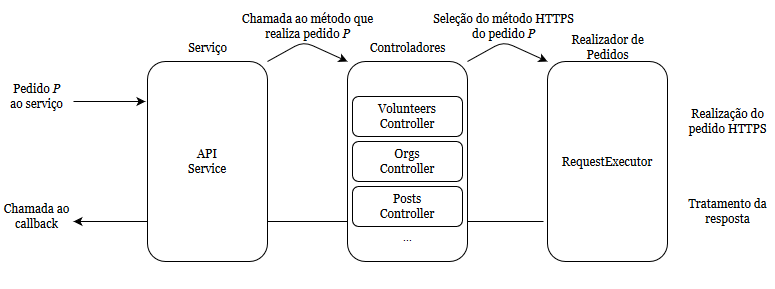
\includegraphics[scale=.42]{mobile_api_architeture}
	\caption{Arquitetura do sub-módulo API}
\end{figure}

O realizador de pedidos trata da implementação dos métodos HTTP suportados pela Web API (GET, POST, PUT, DELETE) de forma genérica, de maneira a que o mesmo possa ser utilizado pelos controladores.

Quando o pedido é concluído, é chamado o \textit{callback} definido pela estrutura que chamou o serviço, que consome a resposta do mesmo, quer esta contenha dados ou apenas sinalize sucesso. A estrutura que efetua a chamada ao serviço é também responsável por definir o \textit{callback} a executar em caso de ocorrer um erro durante o pedido.

\subsection{Modelo}

O Modelo é responsável por transformar os dados provenientes do sub-módulo API para conjuntos de DTO (\textit{Data Transfer Object}) que irão ser usados pelo sub-módulo UI para efetuar a sua representação.

\medskip

Este sub-módulo contém também a definição de uma estrutura que realiza \textit{caching} dos dados da aplicação para diminuir o número de pedidos a realizar à API.